The measurements of the spin-parity properties of the Higgs boson make
use of the kinematics of the four leptons in the event, for the
$\PH\to\V\V$ channels.  For a spin-zero resonance, there is no
correlation between the initial state polarization and the final state
kinematic distributions, while for a spin-one or spin-two boson such a
correlation introduces non-trivial dependence of the final state on
the production mechanism.  The techniques to exploit all these
informations are described in
Refs.~\cite{Soni:1993jc,Barger:1993wt,Choi:2002jk,Choi:2002jk,
  Buszello:2002uu,Godbole:2007cn,Keung:2008ve,Antipin:2008hj,Hagiwara:2009wt,
  Gao:2010qx,DeRujula:2010ys,Gainer:2011xz, Bolognesi:2012mm,
  Chen:2012jy,Anderson:2013afp,Gainer:2013rxa}.

\subsection{Kinematics of $\chanHZZ$}
\label{sec:hzzkinematics}
The event selection of $\chanHZZ$ candidates is the same as the one
used to perform the other measurements in this channel, and reported
in ~\cite{Chatrchyan:2013mxa+}. Analogously, the selected candidates
for the $\chanHWW$ are the same as described in
~\cite{Chatrchyan:2013iaa}. For both decay modes, events are triggered
by requiring the presence of two leptons, electrons or muons, and the
offline analysis require four and two lepton candidates (electrons or
muons), respectively, originating from a vertex with the largest $\sum
\pt^2$ of all tracks associated with it.  Electron candidates are
defined by a reconstructed track in the tracking detector pointing to
an energy deposition in the ECAL.  The electron energy is measured
primarily from the ECAL cluster energy, and combined with the track
momentum to improve the energy resolution at low $\pt$.  Muon
candidates are identified by signals of charged-particle tracks in the
muon system that are compatible with a track reconstructed in the
central tracking system.  Electrons and muons are required to be
isolated. Electrons are reconstructed within the geometrical
acceptance, $|\eta| < 2.5$, and for $\PT > 7\GeV$. Muons are
reconstructed within $|\eta| < 2.4$ and $\PT >
5\GeV$~\cite{Chatrchyan:2012xi}.  For the $\chanHgg$ analysis, photons
are identified as ECAL energy clusters not linked to the extrapolation
of any charged-particle trajectory to the ECAL.  Jets are
reconstructed from the PF candidates, clustered with the anti-$k_t$
algorithm~\cite{Cacciari:2008gp, Cacciari:2011ma} with a size
parameter of 0.5, and they are used to categorise events to enhance
gluon fusion or VBF productions. The missing transverse energy vector
$\vmet$ is defined as the negative vector sum of the transverse
momenta of all reconstructed particles (charged or neutral) in the
event, with $\met = |\vmet|$.

For the $\chanHZZ$ decay, events are selected with at
least four identified and isolated electrons or muons.  Each $\PZ\to
\ell^+\ell^-$ candidate originating from a pair of leptons of the same
flavor and opposite charge is required.  The $\ell^+\ell^-$ pair with
an invariant mass, $m_1$, nearest to the nominal $\PZ$ boson mass is
retained and is denoted $\PZ_{1}$ if it is in the range $40 \le m_1
\le 120 \GeV$.  A second $\ell^{+}\ell^{-}$ pair, denoted $\PZ_{2}$,
is required to have $12 \le m_2 \le 120 \GeV$.  At least one lepton
should have $\PT \ge 20 \GeV$, another one $\PT \ge 10 \GeV$ and any
oppositely charged pair of leptons among the four selected must
satisfy $m_{\ell\ell} \ge 4 \GeV$. Events are selected in a range
around the observed 125.6~\GeV resonance, $105.6 \le m_{4\ell} \le
140.6 \GeV$.
%
The dominant background, $\Pq\Paq \to \PZ\PZ/\PZ\Pgs$ and $\Pg\Pg \to
\PZ\PZ/\PZ\Pgs$ processes, are evaluated from simulation, while the
reducible background, denoted as $\PZ + X$, is estimated from data
control samples with relaxed lepton identification criteria.
%
The event yields are reported in~~\cite{Chatrchyan:2013mxa}.
%
For this channel, the four-momenta of the $\PH \rightarrow
4\mathrm{\ell}$ decay products carry eight independent degrees of
freedom, which fully describe the kinematic configuration of a
four-lepton system in its center-of-mass frame, except for an
arbitrary rotation around the beam axis. These can be conveniently
expressed in terms of the five angles $\vec\Omega\equiv(\theta^*,
\Phi_1, \theta_1, \theta_2, \Phi)$, the invariant masses of the
dilepton pairs, $m_{1}$ and $m_{2}$, and of the four-lepton system,
$m_{4\ell}$.  We give the distribution of two of these kinematic
variables $(m_1, m_{4\ell}$, in data and simulation, in
Fig.~\ref{fig:hzzkinematics}. The $m_1$ distribution is presented
range of $121.5 - 130.5$ GeV to enhance the signal purity, with the
expectations for the SM background, the Higgs boson signal, and some
characteristic alternative spin-zero scenarios.

%%%%%%%%%%%%%%%%%%%%%%%%%
\begin{figure}[!p]
\begin{center}
\centerline{
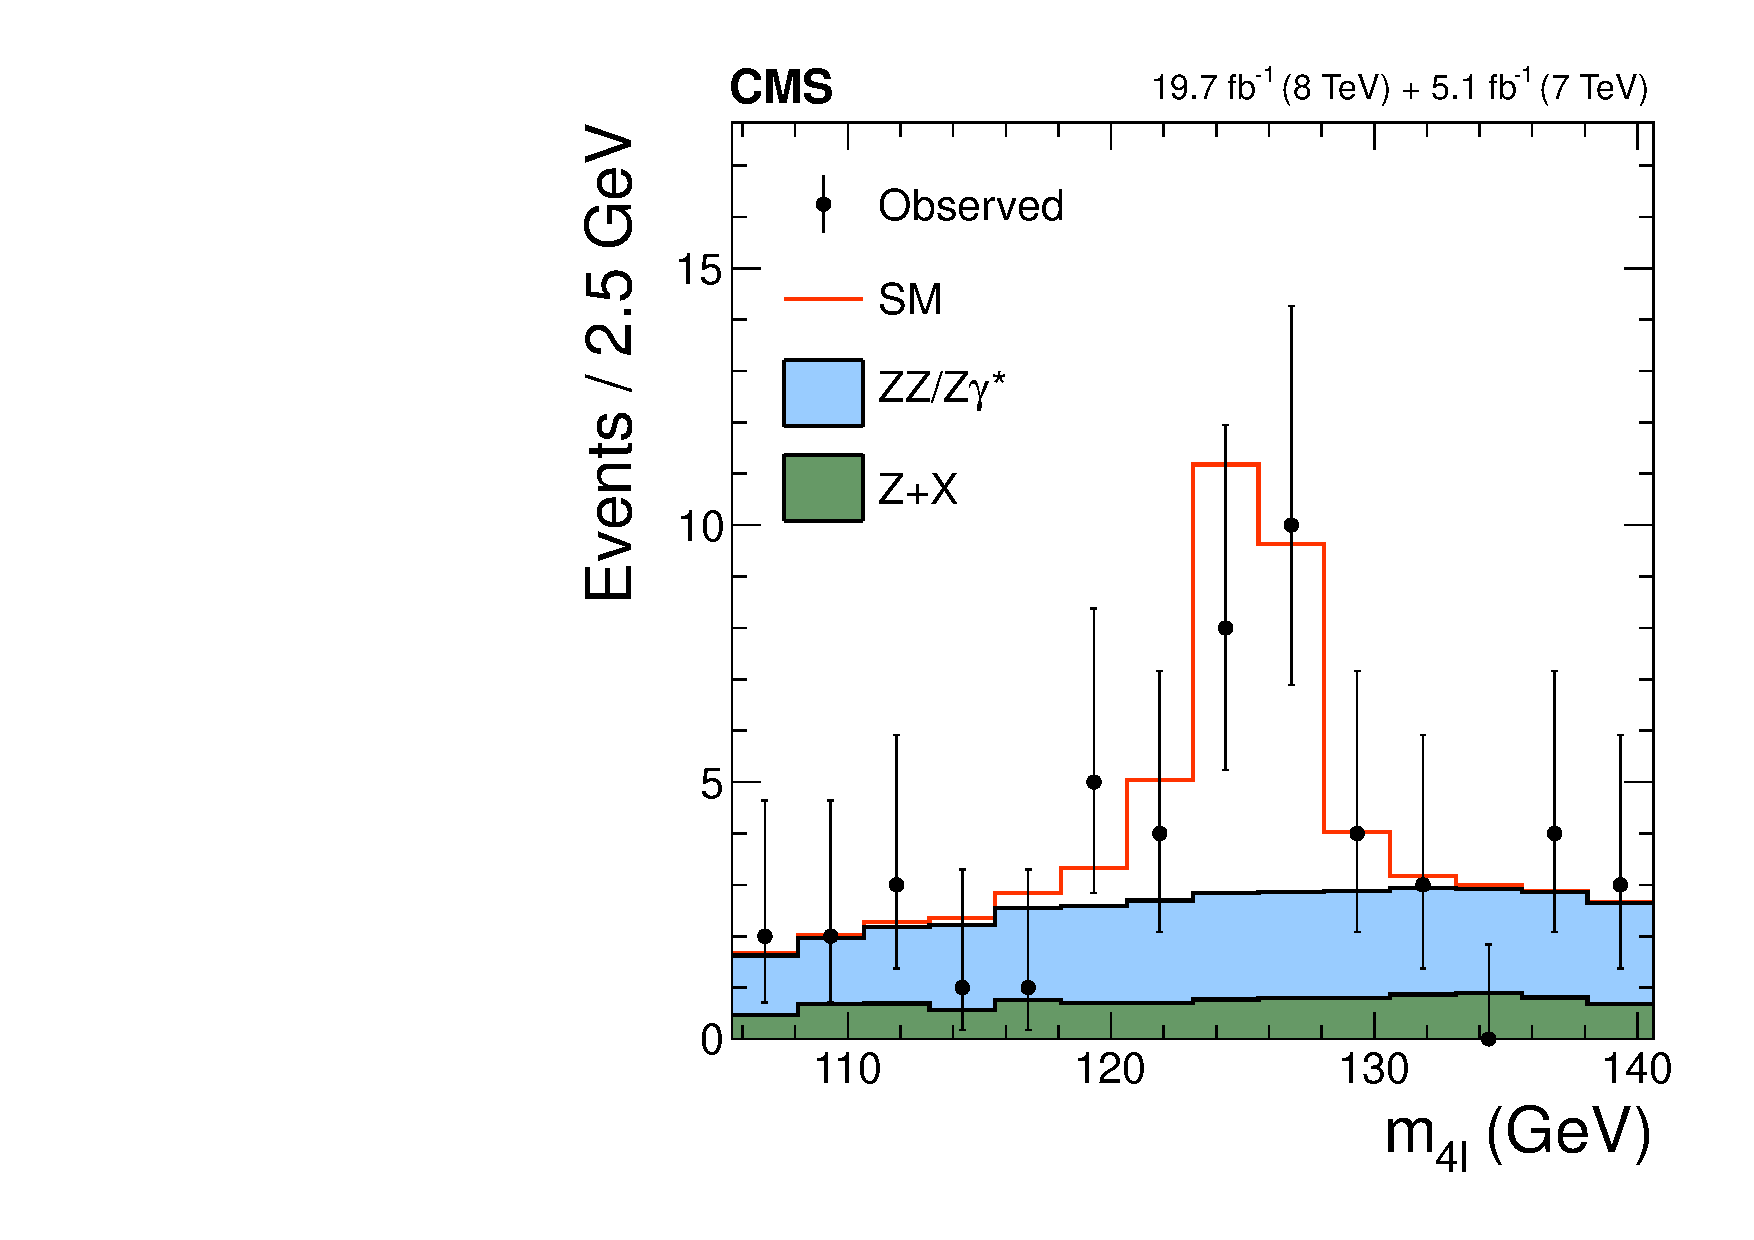
\includegraphics[width=0.50\linewidth]{figures/cCompare_DataMC_AllTeV_ZZMass.pdf}
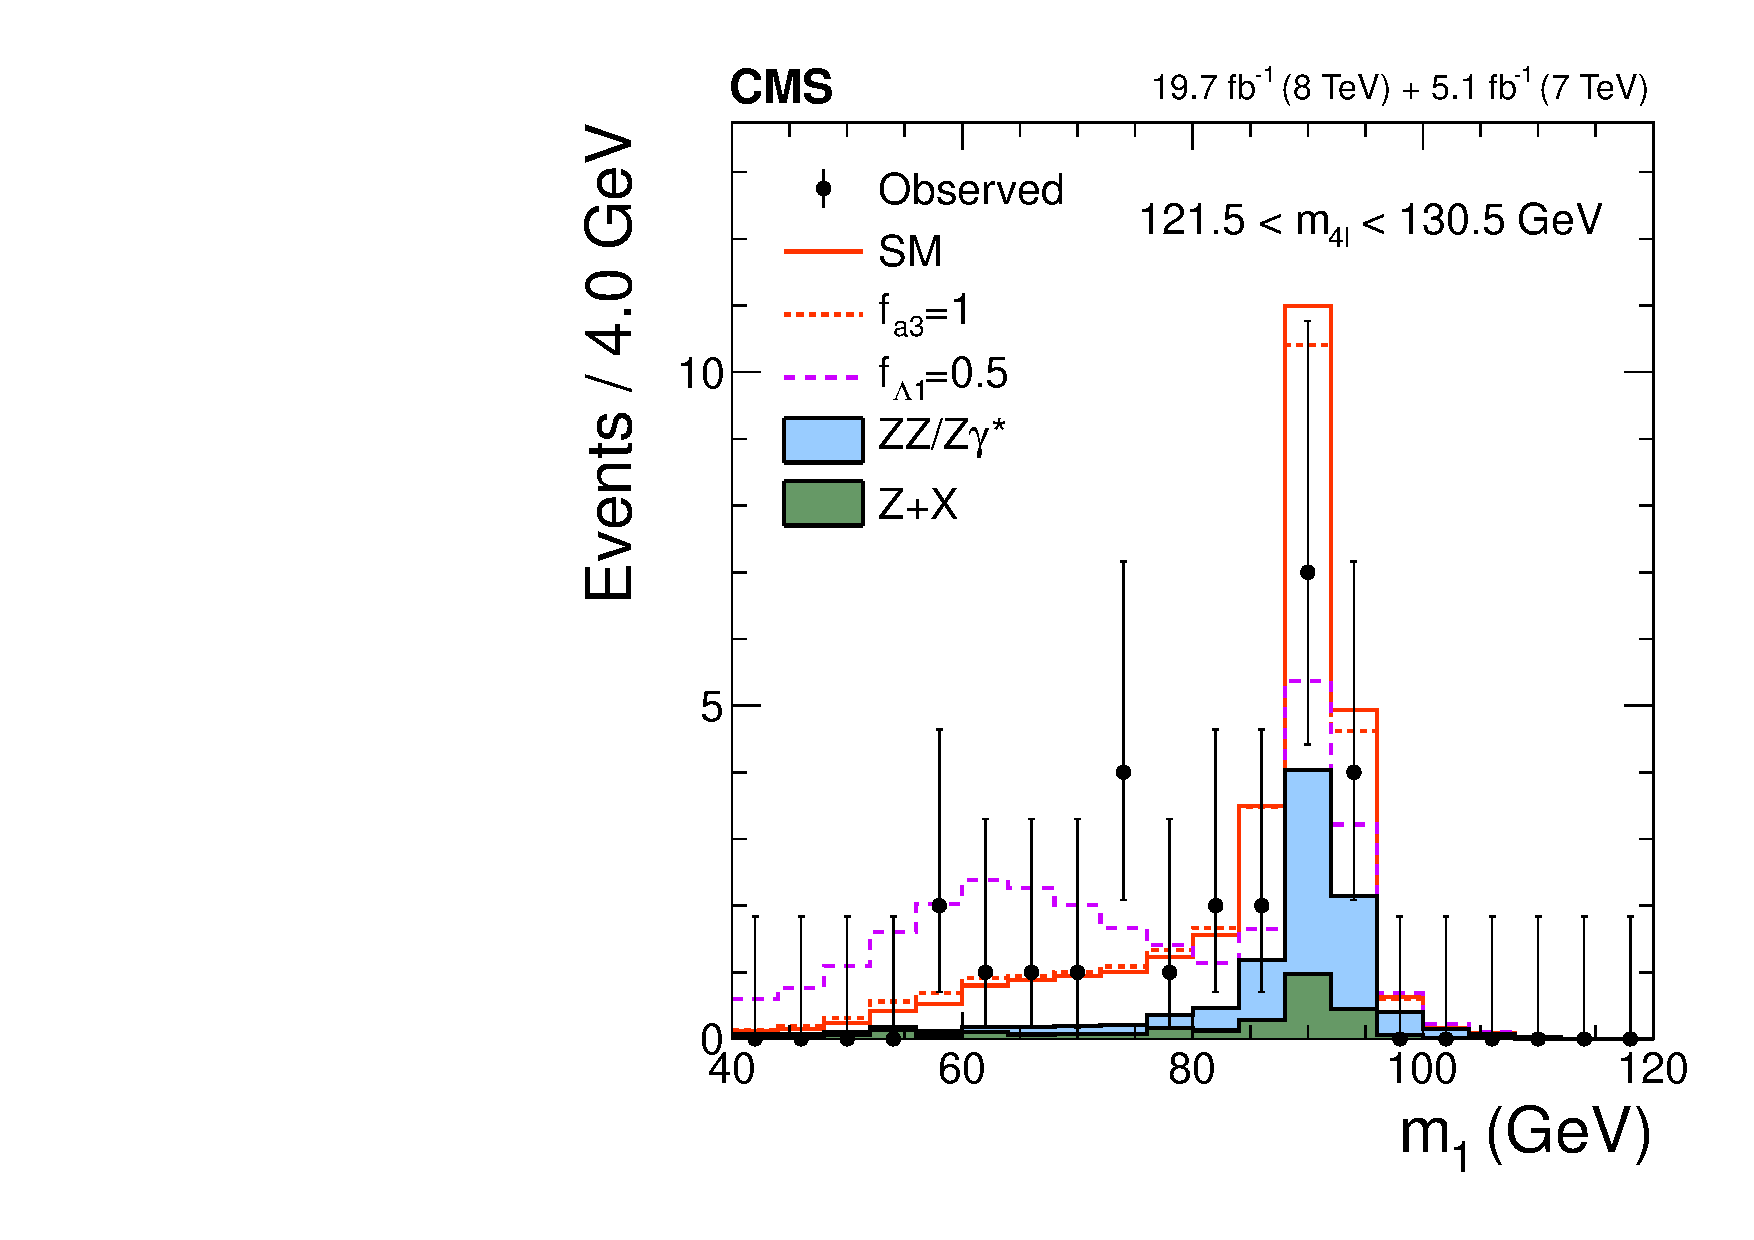
\includegraphics[width=0.50\linewidth]{figures/cCompare_DataMC_AllTeV_Z1Mass_SignalEnriched.pdf}
}
\caption{ Distributions of two out of the eight kinematic observables
  used in the $\chanHZZ$ analysis: $m_{4\ell}$, $m_1$.  Distributions
  show the observed data (points with error bars), the expectations
  for the SM background (shaded areas), the SM Higgs boson signal
  (open areas under the solid histogram), and the alternative
  spin-zero resonances (open areas under the dashed histograms).  The
  mass of the resonance is taken to be 125.6 GeV and the SM cross
  section is used.  The $m_1$ distribution is presented with the
  requirement $121.5 < m_{4\ell} < 130.5$ GeV.  
\label{fig:hzzkinematics} }
\end{center}
\end{figure}
%%%%%%%%%%%%%%%%%%%%%%%%%

One of the approaches pursued in this channels is to parameterise the
multidimensional distributions as a function of the parameters of
interests, which in this approach are the anomalous couplings. Given
the difficulty to populate eight-dimensional distributions for
components that cannot be described analytically, like the
$\Pg\Pg\to\PZ\PZ/\PZ\Pgs$ and $Z+$X processes, this approach is only
pursued for some of the measurements for a spin-zero resonance.
The analytic parameterization is the product of the differential decay cross section, 
$d\sigma_{4\ell}$, and the production spectrum, $W_{\mathrm{prod}}$, written as
%
\begin{eqnarray}
\label{eqn:gen_pdf}
{\cal P}(\vec{p}_\mathrm{T},Y,\Phi^*, \vec{x} | \vec{\zeta}) =
W_{\mathrm{prod}}(\vec{p}_\mathrm{T},Y,\Phi^*,\hat{s}) \times \\ \nonumber
\frac{d\sigma_{4\ell}(m_{4\ell},m_1, m_2, \vec\Omega | \vec{\zeta})}{dm_1^2dm_2^2d\vec\Omega}\,, 
\end{eqnarray}
%
where $\vec{p}_\mathrm{T}$, $Y$, and $\Phi^*$ are the transverse
momentum, rapidity, and azimuthal orientation of the four-lepton
system, and $\hat{s}=m_{4\ell}^2$ is the center-of-mass energy of the
parton-parton system. This probability is converted into
detector-level observables through transfer functions,
$T({\vec{x}^{\prime\mathrm{R}}} | \vec{x}^{\prime\mathrm{G}})$,
describing the detector response to produced leptons. Due to the
excellent angular resolution of the CMS tracker, the effect of the
resolution on the lepton direction is neglected.


The eight-dimensional analysis can be reduced to a three-dimensional
one by storing the full kinematic information in a discriminant
designed for the separation of either background (${\cal D}_{\rm
  bkg}$), the alternative signal components (${\cal D}_{J^P}$), or
interference between those components (${\cal D}_{\rm int}$).  The
construction of the kinematic discriminants follows the matrix element
likelihood approach ({\sc MELA}
package~\cite{Chatrchyan:2012ufa,Gao:2010qx,Bolognesi:2012mm,Anderson:2013afp}),
where the probabilities for an event are calculated using the LO
matrix elements as a function of angular and mass observables.  The
$\JHUGEN$ matrix elements are used for the signal, $\Pg\Pg$ or
$\qqbar\to \X\to \PZ\PZ$ / $\PZ\Pgs$ / $\Pgs\Pgs\to4\ell$, and $\MCFM$
matrix elements for the background, $\Pg\Pg$ or $\qqbar\to\PZ\PZ$ /
$\PZ\Pgs$ / $\Pgs\Pgs$ / $\PZ\to 4\ell$.
%
To remove the dependence of the spin-one and spin-two discriminants on
the production model, the probability ${\cal P}^{\rm kin}$ is averaged
over the two production angles $\cos\theta^*$ and $\Phi_1$, or
equivalently the signal matrix element squared is averaged over the
polarization of the resonance~\cite{Anderson:2013afp}, defining two
production-mechanism-independent discriminants, equivalent to the ones
for a spin-zero resonance: ${\cal D}^{\rm dec}_{\rm bkg}$ and ${\cal
  D}^{\rm dec}_{J^P}$.

\subsection{Kinematics of $\chanHWW$}
\label{sec:hwwkinematics}

For the $\chanHWW$ decay, events with exactly one electron and one
muon are selected, passing tight identification criteria to suppress
the reducible background from $\wjets$ processes, as described in
Ref.~~\cite{Chatrchyan:2013iaa}.  The events with two same-flavor
leptons are not considered for the high Drell-Yan background.  The
$\mathrm{e}\mu$ pair is required to have an invariant mass above
$12\GeV$, and a \pt above $30\GeV$. Events are also required to have
\textit{projected}~$\MET$ above 20~$\GeV$, as defined in
Ref.~\cite{Chatrchyan:2013iaa}. Signal events with exactly zero or one
jet reconstructed satisfying $\et>30~\GeV$ and $|\eta|<$~4.7 are
dominated by gluon fusion Higgs boson production, while events with
exactly two jets are dominated by VBF production.

The main backgrounds, the non-resonant $\PW\PW$ production and
top-quark production ($\ttbar$ and $\tw$ processes, are estimated from
data.  The reducible background arising from misidentified leptons
from $\wjets$ processes is estimated from a data control sample with
loosened lepton identification. The contribution from the $\wgamma^*$
process is also estimated from data with three leptons. The residual
minor backgrounds from triboson ($\V\V\V$) and sub-dominant $\PW\PZ$
and $\PZ\PZ$ are estimated from simulation.
%
The event yields observed in data and the expectation from 
the different processes are given in Ref.~\cite{Chatrchyan:2013iaa}.
%
As a difference with the $\chanHZZ$ case, only partial reconstruction
of the four leptons is possible in this channel, because of the two
undetected neutrinos. Two distributions are used in this case,
summarizing the kinematics of the two detected charged leptons and the
$\met$ of the event: the transverse mass of the final state ($\mth$),
defined as $\mth^2 = 2 \ptll \met (1-\cos\delphillmet)$, and the
dilepton mass ($\mll$) which is one of the most discriminating
kinematic variables for a Higgs boson with low mass, and it is also
correlated to the spin via the azimuthal opening angle between the
two leptons. 
%
The signal region is defined by $\mll < 200$~GeV, and $60 \leq \mth
\leq 280~\GeV$.  The distributions of these observables for data, an
expected SM Higgs signal and backgrounds are presented in
Fig.~\ref{fig:hwwkinematics} for events with no reconstructed jets,
which is the most sensitive category of this analysis.
%

%%%%%%%%%%%%%%%%%%%%%%%%%
\begin{figure}[!p]
\begin{center}
\centerline{
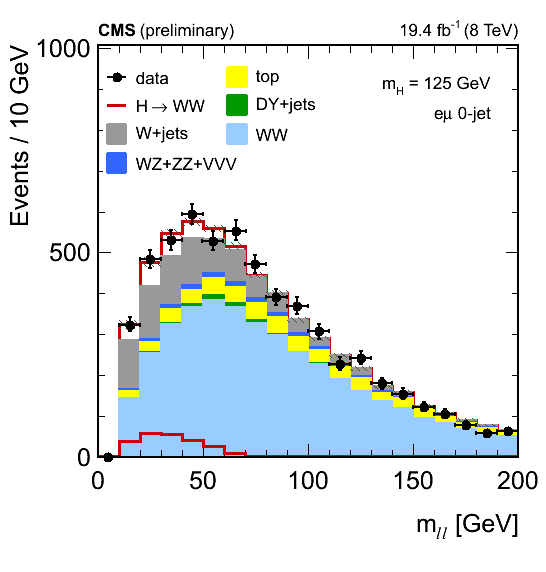
\includegraphics[width=0.50\linewidth]{figures/wwpresel_0j_mh125_massll.png}
~~~~~
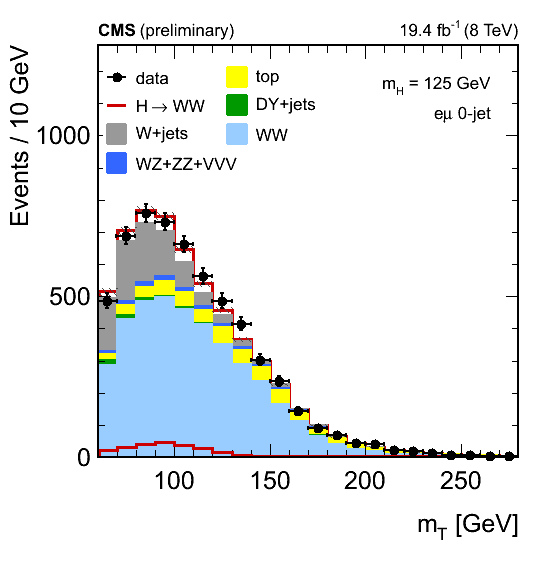
\includegraphics[width=0.50\linewidth]{figures/wwpresel_0j_mh125_mt.png}
}
\caption{ 
  Distributions of the two kinematic observables
  used in the $\chanHWW$ analysis: $\mll$, $\mth$.  Distributions
  show the observed data (points with error bars), the expectations
  for the SM background (filled areas), the SM Higgs boson signal
  (open areas on top of the solid histogram).  The
  mass of the resonance is taken to be 125 GeV and the SM cross
  section is used.  Events with zero jets are shown.  
\label{fig:hwwkinematics} }
\end{center}
\end{figure}
%%%%%%%%%%%%%%%%%%%%%%%%%


\subsection{Kinematics of $\chanHgg$}
\label{sec:hggkinematics}

For this decay channel, the kinematics of the di-photon events are
defined by the mesurement of the photon energy and position in the
ECAL. The selection for the spin-parity analysis is described in
Ref.~\cite{Khachatryan:2014ira}. The cosine of the scattering angle in
the Collins--Soper frame, $\cos\theta^*$, is used to discriminate
between the spin hypotheses.  The angle is defined in the diphoton
rest frame as that between the collinear photons and the line that
bisects the acute angle between the colliding protons:
%
\begin{equation}
  \costhetastar=2\times\frac{E^{\gamma2}p^{\gamma1}_{z}-E^{\gamma1}p^{\gamma2}_{z}}{\mgg\sqrt{\mgg^{2}+(\ptgg)^{2}}},
\end{equation}
%
where $E^{\gamma1}$ and $E^{\gamma2}$ are the energies of the leading
and subleading photons, $p^{\gamma1}_{z}$ and $p^{\gamma2}_{z}$ are
the $z$ components of their momenta, and $\mgg$ and $\ptgg$ are the
invariant mass and transverse momentum of the diphoton system.  In the
rest frame of a spin-0 boson the decay photons are isotropic, and so,
before the acceptance requirements, the distribution of \costhetastar
is uniformly flat under the SM hypothesis.  In general this is not
the case for the decay of a spin-2 particle.  Within each diphoton
class, the events are categorized in five $|\cos\theta^*|$ bins to
discriminate between the different spin hypotheses, and in several
$(\eta, R_9)$ categories to enhance the sensitivity.
%

